% Exact within-release display, based on SUCCESS run 38388066957.
\begin{figure}[ht]
\centering
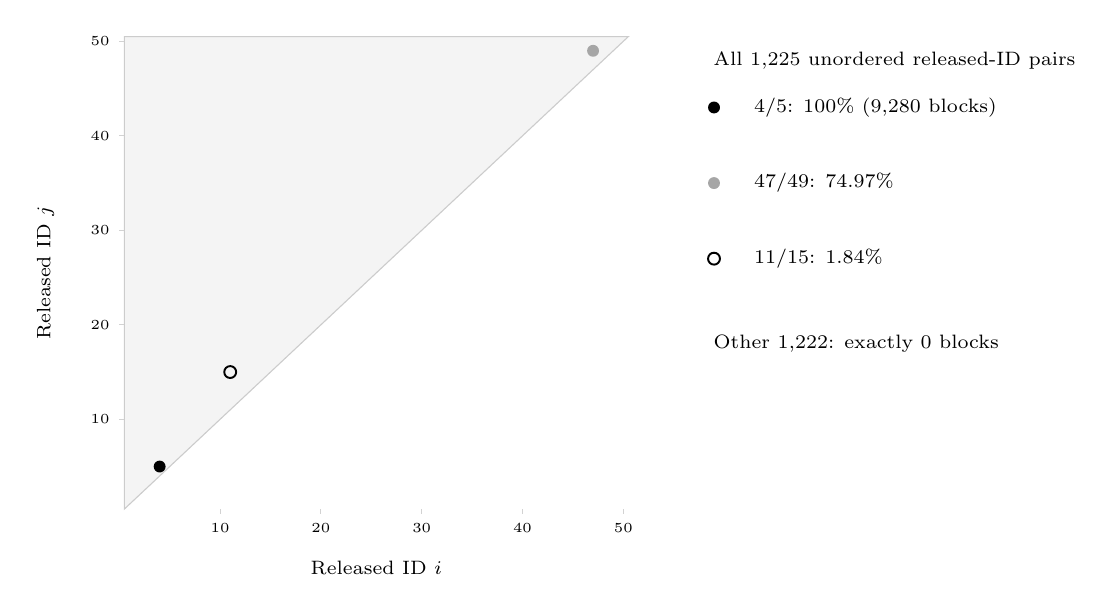
\begin{tikzpicture}[x=.128cm,y=.120cm]
  % Triangular comparison domain: x=i, y=j, 1<=i<j<=50.
  \fill[gray!9] (0.5,0.5)--(0.5,50.5)--(50.5,50.5)--cycle;
  \draw[gray!40,line width=.4pt] (0.5,0.5)--(0.5,50.5)--
     (50.5,50.5)--cycle;
  \foreach \v in {10,20,30,40,50} {
    \draw[gray!35,line width=.35pt] (\v,.5)--(\v,0);
    \node[anchor=north,font=\tiny] at (\v,0) {\v};
    \draw[gray!35,line width=.35pt] (.5,\v)--(0,\v);
    \node[anchor=east,font=\tiny] at (0,\v) {\v};
  }
  \node[font=\scriptsize,anchor=north] at (25.5,-4) {Released ID $i$};
  \node[font=\scriptsize,rotate=90,anchor=south] at (-5.5,25.5) {Released ID $j$};
  % Black = full 29 EEG streams, dark grey = >=50% native EEG blocks,
  % open = <2% nonzero exact blocks.
  \fill[black] (4,5) circle [radius=2.15pt];
  \fill[gray!70] (47,49) circle [radius=2.15pt];
  \draw[black,line width=.7pt] (11,15) circle [radius=2.15pt];
  \begin{scope}[shift={(58,43)}]
     \node[font=\scriptsize,anchor=west] at (0,5)
       {All $1{,}225$ unordered released-ID pairs};
     \fill[black] (1,0) circle [radius=2.15pt];
     \node[font=\scriptsize,anchor=west] at (4,0)
       {4/5: 100\% (9,280 blocks)};
     \fill[gray!70] (1,-8) circle [radius=2.15pt];
     \node[font=\scriptsize,anchor=west] at (4,-8)
       {47/49: 74.97\%};
     \draw[black,line width=.7pt] (1,-16) circle [radius=2.15pt];
     \node[font=\scriptsize,anchor=west] at (4,-16)
       {11/15: 1.84\%};
     \node[font=\scriptsize,anchor=west] at (0,-25)
       {Other $1{,}222$: exactly 0 blocks};
  \end{scope}
\end{tikzpicture}
\caption{Public digital content overlap among 50 published Liu2024
IDs in NEMAR v1.0.3. One point per unordered released-ID pair,
$x=i$, $y=j$, $i<j$. Filled black indicates full 29-EEG-channel
and aligned storage-block equality, dark gray indicates partial
exact aligned storage-block overlap above 50\%, and open indicates
a nonzero fraction below 2\%. The unmarked pale triangular region
contains 1,222 pairs with no same-channel, same-record exactly
equal EEG storage blocks. These are \emph{native EDF storage
blocks, not clinical trials}; digital equality does not assign
patient identity or prove acquisition reuse. Values from the
50-full-file checksum-verified external-distributor rerun
(see Table~\ref{tab:p2-nemar-full50}).}
\label{fig:p2-all50-digital-reuse-matrix}
\end{figure}
